\documentclass[a4paper,10pt,oneside,fleqn]{jsarticle}
%
\usepackage{amsmath,amssymb,bm}
\usepackage{bm}
\usepackage{graphicx}
\usepackage{ascmac}
\usepackage{makeidx}
\usepackage{txfonts}
\usepackage{indentfirst}
\usepackage{indent}
\usepackage{booktabs}
\usepackage{comment}
\usepackage{cite}
\usepackage{subfigure}
\usepackage{float}
\usepackage{alltt}
\usepackage{eclbkbox,fancybox}
\usepackage{fancyhdr} \pagestyle{fancy}
%
\newcounter{program}
%\bkcounttrue
\newenvironment{program}%
{\vspace{0.5\baselineskip}\VerbatimEnvironment%
%\begin{breakbox}\setlength{\baselineskip}{0pt}\begin{Verbatim}}%
\begin{breakbox}\setlength{\baselineskip}{.25\normalbaselineskip}\begin{Verbatim}}%
{\end{Verbatim}\end{breakbox}\vspace{0.8\baselineskip}}

%
\makeindex
%
\newcommand{\diff}{\mathrm{d}}  %微分記号
\newcommand{\divergence}{\mathrm{div}\,}  %ダイバージェンス
\newcommand{\grad}{\mathrm{grad}\,}  %グラディエント
\newcommand{\rot}{\mathrm{rot}\,}  %ローテーション
%
\setlength{\textwidth}{\fullwidth}
\setlength{\textheight}{44\baselineskip}
\addtolength{\textheight}{\topskip}
\setlength{\voffset}{-0.6in}
\setlength{\mathindent}{1.5cm} %数式のインデント設定
\setcounter{secnumdepth}{2} %subsectionまで番号付け
\setcounter{tocdepth}{4} %目次の深さ設定
\renewcommand\citemid{; } %citeのオプション
%
\title {\huge \textbf{FrontFlow / violet Cartesian}}

\author{Kenji ONO, AICS, RIKEN\\ keno@riken.jp}

\date{\today}

%fancy header
\rhead{FFVC}

\graphicspath{{./}}

%
\begin{document}

\maketitle


%%
\section{ディレクトリ・ファイル構成(Directories and files)}

ffvc-x.x.x.tar.gzを解凍すると,以下のようなファイル構成になります\footnote{doxygenディレクトリについては,doxygenファイルを生成するために必要な設定ファイルのみを提供しています.Confディレクトリ内でmakeを実行すると各ディレクトリにdoxygenファイルが生成されます.}.

{ \small
\begin{program}
ffvc-x.x.x
  |
  +- BUILD                        アプリケーションのコンパイル方法のメモ
  +- COPYING                      コピーライト
  +- README                       最初に見るべきファイル
  +- RELEASE                      リリース情報
  |
  +- bin                          実行モジュールの配置ディレクトリ
  |
  +- doc                          ドキュメント
  |   +- ffvc_ug.pdf              FFV-Cソルバーのユーザガイド
  |   
  +- doxygen                      Doxygenドキュメントディレクトリ
  |   +- FFV                      FFVクラスのドキュメント
  |   +- Conf                     Doxygenファイルを生成するための設定ファイル
  |   +- FB                       FBクラスのドキュメント
  |   +- IP                       Intrinsicクラスのドキュメント
  |
  +- example                      例題
  |   +- Cavity_binary            三次元のキャビティフロー例題(バイナリモデル)
  |   +- Cavity_cut               三次元のキャビティフロー例題(カット情報モデル)
  |   +- LDC                      辺長比1:1:2のキャビティフロー例題(実験値との比較)
  |   +- PMT                      性能測定用例題
  |   +- Sphere                   球周りの流れ例題
  |
  +- src                          ソースコードディレクトリ
      +- Cutlib-x.x.x             カットライブラリ
      +- F_CORE                   Fortranのコアプログラム(Binary版)
      +- F_VOF                    VOFクラスのFortranファイル
      +- FB                       FlowBaseクラス(ユーザー定義クラス群)
      +- FFV                      FFV-Cソルバ
      +- IP                       組み込み例題クラス群
      +- PMlib-x.x                性能測定ライブラリ
      +- Polylib-x.x.x            ポリゴン管理ライブラリ

\end{program}
}

\clearpage

%%
\section{ビルド手順 (How to build)}
ビルドは,OpenMPI, TextParser, CPMlib, FFVの順序で行います.

%
\subsection{必要な外部ライブラリ (External libraries)}

次のライブラリが必要です.TextParser, CPMlibについては,本パッケージ内に同梱しています.

\begin{itemize}
\item OpenMPI (1.6.2)
\item TextParser (1.1)
\item CPMlib (1.0.6)
\end{itemize}


%
\subsection{コンパイラ,ビルドツール (Compiler and build tools)}

\begin{itemize}
\item コンパイラ\\
利用するコンパイラは,Intel Compiler C/C++, Fortran XE Intel(R) 64, Version 13.0.0.088を利用しています.
gcc, gfortran, xlc/c++, xlfでのコンパイルも可能です.

\item ビルドツール\\
make, auto toolsを利用します.一部autotoolsが使えない場合には,手動によるmakeで対応します.

\end{itemize}
   
   
%
\subsection{ビルド方法 (Build)}
簡単な手順を以下に示します.詳細については,\verb|ffvc_ug.pdf|のインストールをご覧ください.

\begin{enumerate}

\item TextParserのインストール\\
\verb|TextParser-x.x.tar.gz|を展開し,トップディレクトリの\verb|config_tp.sh|を実行します.

{\small
\begin{program}
$ configure_tp.sh /usr/local/TextParser
$ make
$ sudo make install または make install
$ make distclean
\end{program}
}


\item CPMlibのインストール\\

\verb|CPMlib-x.x.x.tar.gz|を展開し,トップディレクトリの\verb|config_cpm.sh|を実行します.

{\small
\begin{program}
$ configure_cpm.sh /usr/local/cpm
$ make
$ sudo make install または make install
$ make distclean
\end{program}
}

configureがうまくいかない場合は,\verb|Makefile_hand|を使い,コンパイルします.

{\small
\begin{program}
$ make -f Makefile_hand mpi
\end{program}
}


\item FFV-Cのコンパイル\\

\begin{enumerate}

\item 一括コンパイル\\
Polylib, Cutlib, PMlibがFFVディレクトリと同じ階層に配置されていることが必要です.

{\small
\begin{program}
$ make depend
$ make
\end{program}
}

\item 個別にコンパイル\\
以下の順序でコンパイルを行います.
コンパイルをやり直す場合には,\verb|make clean, make allclean|を実行します.

\begin{enumerate}

\item Polylib\\
\verb|Makefile|のマクロ変数を指定し,コンパイルします.

{\small
\begin{program}
$ make depend
$ make
\end{program}
}

\item Cutlib\\
\verb|Makefile|のマクロ変数を指定し,コンパイルします.

{\small
\begin{program}
$ make depend
$ make
\end{program}
}

\item PMlib\\
\verb|Makefile|のマクロ変数を指定し,コンパイルします.

{\small
\begin{program}
$ make depend
$ make
\end{program}
}

\item FFV-C\\
\verb|make_setting|のマクロ変数を指定し,コンパイルします.

{\small
\begin{program}
$ make depend
$ make
\end{program}
}

\end{enumerate}
\end{enumerate}
\end{enumerate}  



%%
\section{実行手順 (How to run)}

%
\subsection{入力ファイル、設定ファイル (Input files)}

実行に必要なファイルは計算対象とする問題により異なりますが,組み込み例題の場合にはパラメータファイルのみです.
パラメータファイルの例が,example配下のディレクトリにあります.
パラメータファイルの指定の詳細については,ユーザガイドをご覧ください.
   
   
%
\subsection{出力ファイル (Output files)}

FFV-Cソルバーを実行すると,\textbf{表\ref{tbl:logfiles}}に示すファイルが生成されます.
また,logファイルについては,Logセクションで生成の有無を指定します.
全ての出力ファイルは,パラメータファイルにより指定できます.


\begin{table}[htdp]
\caption{実行時に生成されるファイル}
\begin{center}
\small
\begin{tabular}{lll}\toprule
カテゴリ & ファイル名 & 出力内容\\ \midrule
解析条件情報 & \verb|condition.txt| & 計算条件,前処理,ソルバー起動時のログ\\
領域情報 & \verb|DomainInfo.txt| & 並列計算時の計算領域の分割に関する情報\\ 
性能情報 & \verb|profiling.txt| & 実行時間サンプリング出力ファイル\\ \hline
基本履歴 & \verb|history_base.txt| & ステップ数,時刻,反復回数,収束状況などの情報\\
コンポーネント履歴 & \verb|history_compo.txt| & 内部境界のモニタ情報\\
流量収支履歴 & \verb|history_domainflux.txt| & 計算外部領域における流入出流量,平均速度の情報\\
反復履歴 & \verb|history_iteration.txt| & 反復解法の収束履歴\\ 
サンプリング履歴 & \verb|sampling.txt| & サンプリング指定時の出力ファイル\\ 
壁面情報履歴 & \verb|history_log_wall.txt| & 壁面に関する情報の履歴\\ \hline
瞬時値データ & \verb|vel_*.sph| & 速度の瞬時値\\
& \verb|prs_*.sph| & 圧力の瞬時値\\
& \verb|tmp_*.sph| & 温度の瞬時値\\
平均値データ & \verb|vela_*.sph| & 速度の時間平均値\\
& \verb|prsa_*.sph| & 圧力の時間平均値\\
& \verb|tmpa_*.sph| & 温度の時間平均値\\
派生データ & \verb|tp_*.sph| & 全圧\\
& \verb|vrt_*.sph| & 渦度\\
& \verb|hlt_*.sph| & ヘリシティ\\
& \verb|i2vgt_*.sph| & 速度勾配テンソルの第2不変量\\ 
\bottomrule
\end{tabular}
\end{center}
\label{tbl:logfiles}
\end{table}

   

%
\subsection{サンプルデータ (Sample data)}
サンプルデータとして,exampleディレクトリ配下にあるPMTをご利用ください.
PMTの例題は,並列性能の測定を行う例題でファイルは出力しません.
反復法の上限値を変更することにより,実行時間を調整することが出来ます.
   
%
\subsection{実行方法 (Run)}
実行方法は,\verb|pm_1.tp|を入力パラメータファイルとして,以下のようになります.

{\small
\begin{program}
$ ffvc pm_1.tp
\end{program}
}
  

%
\subsection{参考情報 (Reference information)}
下記のGlobal\_Voxelの要素数を変更することにより,メモリサイズ,ファイルサイズ,計算時間が変わります.

{\small
\begin{program}
DomainInfo {
  Global_origin   = (-0.5, -0.5, -0.5   )
  Global_region   = (1.0,  1.0,  1.0    )
  Global_voxel    = (128   , 128   , 128   )
  ActiveSubDomain_File = ""
}
\end{program}
}

上記の分割数でのweak scalingの結果を\textbf{図\ref{fig:flops}}に示します.
実行時間は140-160秒の範囲です.

\begin{figure}[htbp]
\begin{center}
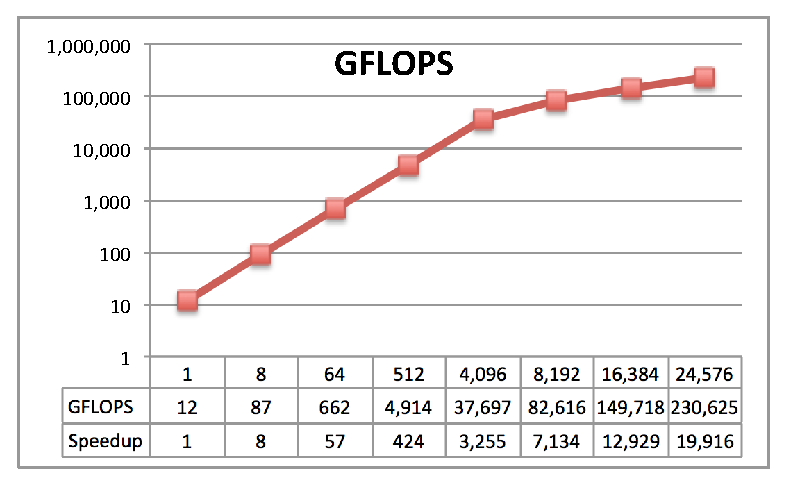
\includegraphics[width=10cm,clip]{performance.eps}
\end{center}
\caption{PMTクラスのweak scaling実行性能.}
\label{fig:flops}
\end{figure}


%%
\section{検証手順 (How to validate)}
暫定的な検証として,example/PMT/history\_base.txtの内容とdiffをとって比較してください.


%
\subsection{検証プログラム (Test program)}

   (検証プログラムの内容説明)

%
\subsection{検証方法 (Run test program)}

   (検証プログラムの具体的な実行方法、実行結果の解釈についての説明)



%
%\bibliographystyle{junsrt}
%\bibliography{tn1}

\newpage
\printindex
%
%
\end{document}